\chapter{Desarrollo de Pasantías}
\label{capitulo3}
\lhead{Capítulo 3. \emph{Diseño del sistema}}

\section{Estado del Arte}

En esta etapa del proyecto se realizó una investigación sobre los conceptos fundamentales del sistema a implementar. Las definiciones estudiadas fueron: el protocolo HTTP, los URIs, detector de intrusiones (IDS), modelo de Markov y SSM.
El resumen de esta investigación se encuentra en el capítulo \ref{capitulo2} del presente trabajo.

\section{Análisis de Bro}

En esta etapa del proyecto se descargó, se instaló y se estudio la herramienta Bro y su lenguaje de ``scripting''. Bro, es la herramienta principal que se utilizó en la implementación del sistema. Un resumen de esta y de su lenguaje de programación se encuentra en la sección \ref{ssec:Bro}.

\section{Diseño de la Arquitectura del Sistema}

Esta sección tiene la intención de mostrar la visión general del modelado del sistema que se realizó a partir de las bases teóricas. Aquí, se explicará la arquitectura, el diseño y el modo en el que el IDS basado en SSM interactuará con Bro. Además, se detallaran las salidas y los datos de configuración
que va a considerar el sistema para su correcto funcionamiento.

\subsection{Arquitectura del Sistema}

La arquitectura del detector de intrusiones que se muestra en el presente trabajo se basa en una arquitectura modular la cual está conformada por tres modulo. Un modulo para realizar la segmentación de los URIs, otro  para realizar la evaluación y un tercero para realizar el entrenamiento.

A grandes rasgos, el módulo de segmentación, se encargará de tomar los URIs previamente filtrados de las solicitudes de tipo HTTP/GET, lo normalizará y lo segmentará de la forma en la que se explicó en el apartado de ``segmentación'' de la sección \ref{sec:delimitadores}.

Por otra parte, el modulo de evaluación se encargará de evaluar la probabilidad de generación de cada uno de los segmentos del URI generados por el módulo de segmentación para al final decidir si el URI de la solicitud enviada al servidor web es anómalo o no.

Por último, el modulo de entrenamiento será el encargado de crear el modelo de normalidad del sistema. Para esto, el sistema recibirá solicitudes libres de ataques e irá calculando la probabilidad de aparición de cada una de las palabras que aparecen en las mismas.

Tanto el modulo de evaluación, como el modulo de entrenamiento son dependientes del modulo de segmentación ya que requieren de los segmentos de URI generados por eso para realizar su trabajo. 

La arquitectura del sistema queda detallada en la figura \ref{fig:arquitectura}.

\begin{figure}[!htb]
\begin{center}
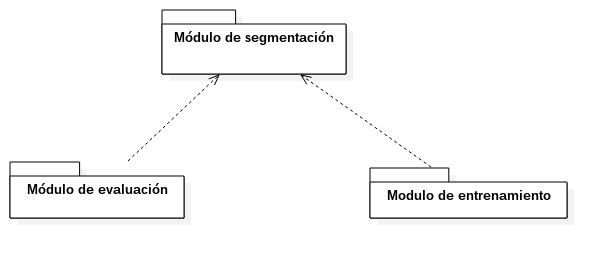
\includegraphics[width=3in]{./img/arquitectura.png}
\caption{Arquitectura del sistema.}
\label{fig:arquitectura}
\end{center}
\end{figure}


Así mismo, es importante mencionar que el sistema contará con varios modos de operación que serán explicados a continuación:

\begin{itemize}
\item Modo evaluación: En este modo de operación solo se activarán los módulos de segmentación y evaluación del sistema. A manera general, esta modalidad, se encargará de recibir los URI previamente extraídos de las peticiones de tipo HTTP/GET, segmentarlos a tráves del módulo de segmentación, para luego evaluar si el mismo es anómalo o no
haciendo uso del módulo de evaluación. El funcionamiento de esta modalidad queda detallado en la figura \ref{fig:modoSistema}.
\item Modo entrenamiento ``Online'': En este modo de operación solo trabajaran los módulos de segmentación y entrenamiento. En esta modalidad el módulo de entrenamiento tomará los segmentos arrojados por el módulo de segmentación, calculará la probabilidad de aparición de los mismos para de esta manera ir modificando un modelo de normalidad previamente establecido. El funcionamiento de esta modalidad queda
detallado en la figura \ref{fig:modoSistema}.
\item Modo entrenamiento ``Offline'': Esta modalidad del sistema en análoga al modo de entrenamiento ``Online''. El único aspecto que diferencia a ambas modalidades es que cuando el sistema funciona en modo ``Offline'' no se toma en cuenta, ni se modifica un modelo de normalidad previamente construido. La salida de este modo de entrenamiento sera un modelo de normalidad construido desde cero.El funcionamiento de esta modalidad queda detallado en la figura \ref{fig:modoSistema}.
\end{itemize}

\begin{figure}[!htb]
\begin{center}
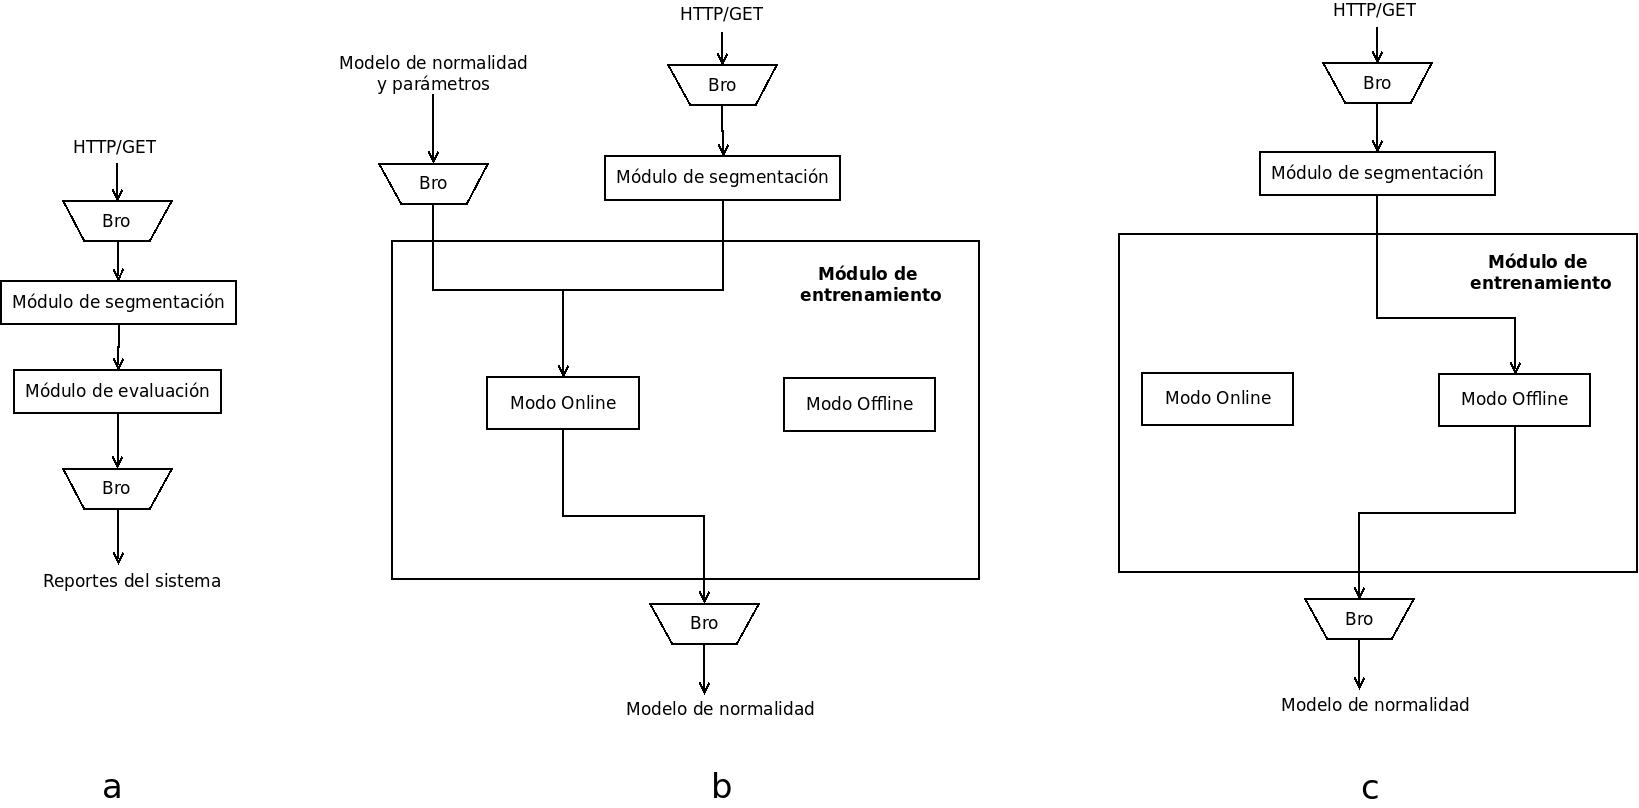
\includegraphics[width=\linewidth]{./img/modoOperacion.jpeg}
\caption{Modo evaluación (a), modo entrenamiento ``Online'' (b), modo entrenamiento ``Offline'' (c).}
\label{fig:modoSistema}
\end{center}
\end{figure}


\subsection{Filtrado de Paquetes HTTP/GET}

Esta funcionalidad se encargará de observar los paquetes de la red y filtrar aquellos de tipo HTTP/GET. Una vez obtenido este tipo de paquetes, esta función extraerá el URI adjunto al mismo.

\subsection{Módulos}

En esta sección se describirán las tareas de cada uno de los módulos que conformar la arquitectura detallada en la figura \ref{fig:arquitectura}, el modo en el que se subdividieron dichas tareas, los datos de entrada y salida, y la interacción que existe entre los mismos.

\subsubsection{Módulo de Segmentación}

El modulo de segmentación es un elemento clave dentro de la construcción del IDS basado en SSM, es por eso que su buen diseño e implementación es importante para el buen funcionamiento del sistema. Este se encarga, como se mencionó anteriormente,de tomar el URI que proviene de la solicitud de tipo HTTP/GET que se le hace al servidor HTTP capturado por Bro, normalizarlo y segmentarlo siguiendo las especificaciones que se explicaron en la sección \ref{sec:delimitadores}. 

Es evidente entonces, que este modulo consta de dos funcionalidades fundamentales: la normalización de los URIs y la segmentación.  La normalización se encargará de tomar el URI de las peticiones HTTP/GET entrantes y codificarlo a formato UTF-8. Normalizar es un paso importante dentro del sistema  ya que se estandarizar la forma en las que están escritos los URIs facilita tanto la evaluación como el entrenamiento en el sistema. Por otra parte, la salida arrojada por esta función de normalización será tomada por la de segmentación, quien a su vez se encargará de segmentar el URI de la forma en la que se explica en la sección \ref{sec:delimitadores}, es decir, el URI se dividirá en las diferentes partes estipuladas en el RFC 3986: el ``host'', la ruta, los argumentos, los valores y el ``fragment''.

 En las base teórica, la segmentación de los URIs se realiza mediante un autómata que se encarga de reconocer (realizar un análisis sintáctico) y evaluar en cada uno de sus estados la probabilidad de generación de cada uno de los segmentos.  No obstante, en la función de segmentación del sistema implementado, esta tarea se modeló mediante un analizador sintáctico que hace uso de una gramática (libre de contexto) de atributos que genera el mismo lenguaje que reconoce el autómata presentado en la figura ~\ref{fig:automata}, es decir, el lenguaje de los URI.

En la figura \ref{fig:arquiSegmentacion} se puede apreciar el diagrama de bloques que refleja el funcionamiento del módulo de segmentación.

\begin{figure}[!htb]
\begin{center}
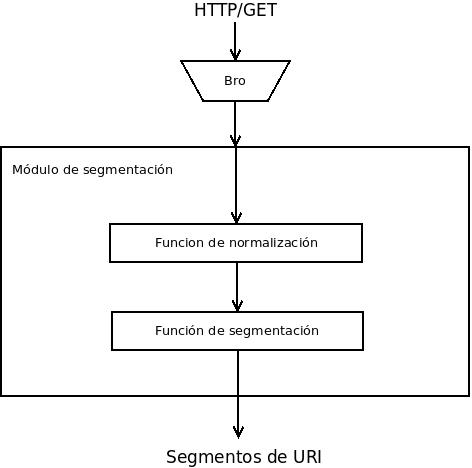
\includegraphics[width=3in]{./img/segArquiCompleta.jpeg}
\caption{Diagrama de bloques del módulo de segmentación.}
\label{fig:arquiSegmentacion}
\end{center}
\end{figure}

\subsubsection{Módulo de Evaluación}
\label{sec:evaluacion}

El módulo de evaluación, es el encargado de evaluar la probabilidad de generación de cada uno de los segmentos del URI otorgados por el modulo de segmentación, dado un modelo de normalidad. Una vez calculadas estas probabilidades, el modulo se encargará de calcular un índice de anormalidad del URI mediante el uso de las formulas descritas en la sección ~\ref{subsec:exprIndice} para luego compararlo con un parámetro $\theta$ (\ref{eq:ClaseU}) y de este modo saber si los segmentos de URI que ingresaron como entrada posee alguna anormalidad o no. Luego de realizar esta evaluación, el modulo se encargara de escribir los reportes del sistema en un ``log''.

El módulo de evaluación, está conformado por dos grandes funcionalidades: una que se encargará de leer el modelo de normalidad y  otra que calculará el índice de anormalidad y evaluará si el mismo es anómalo o no. 

El modelo teórico que fue explicado en la sección ~\ref{sec:modeloSSM} posee elementos como: un conjunto ``S'' de estados, un conjunto ``O'' de símbolos observables que se encuentran en cada estado, una matriz ``A'' que contiene la probabilidad de transición entre estados, un conjunto ``B'' de vectores que contiene la probabilidad de las palabras observadas en cada estado y un vector de probabilidades iniciales. No obstante, los únicos elementos del modelo que se necesitan ingresar en el sistema para que este funcione y realice las tareas de evaluación son: el conjunto ``O'' de símbolos observables que se encuentra en cada estado y el conjunto de vectores ``B''. El conjunto ``B'' es necesario para resolver la expresión \ref{eq:sumB}. Por otra parte, es necesario hacer uso tanto de ``B'' como ``O'' para obtener el valor de $b_{qtot}$ presentado en la ecuación \ref{eq:Pqtot}. Este elemento es sumamente importante para calcular el índice de anormalidad. Por otra parte, será necesario introducir al sistema los valores de probabilidad de fuera de vocabulario (Poov), ya que son necesarios para obtener el valor de $p_{qtot}$, presente en la ecuación \ref{eq:Pqtot}, en caso que una cadena de caracteres del URI que se esté analizando no se encuentre en el conjunto de observaciones ``O''. Además, se requiere el valor del parámetro $\theta$ para evaluar el índice de anormalidad según lo estipulado en la ecuación \ref{eq:ClaseU} .

    Entonces, en conclusión, los parámetros que requieren ser introducidos al sistema de detección de intrusiones para que este funcione de manera correcta son: el conjunto de observaciones de cada estado (O), el conjunto de vectores de probabilidad de las palabras observadas en cada estado ( $B_{S}, B_{P}, B_{A}, B_{V}$ ), los valores de probabilidad de fuera de vocabulario, es decir $P_{oovS}, P_{oovP}, P_{oovA}, P_{oovV}$ y el valor del parámetro $\theta$. Todos estos parámetros serán leídos por la función de lectura del modulo de evaluación.
    
Una vez leídos los parámetros necesarios para que el sistema funcione, estos serán enviados a la función de evaluación junto a los segmentos de URI dados por el módulo de segmentación. Una vez recibidos los datos de entrada, esta función se encargará de hallar el índice de anormalidad ($N_{s}$) mediante la expresión \ref{eq:Ns} para, de este modo compararlo con el parámetro $\theta$ como se indica en \ref{eq:ClaseU}.No obstante, las tareas de calculo y evaluación del índice de anormalidad, fueron subdivididas a su vez, en cuatro funciones. La primera de las funciones será la encargada de calcular tanto el $\varepsilon_{0}$ que aparece en la expresión \ref{eq:sumB} como la sumatoria de los logaritmos de los $p_{qtot}$ que se encuentra en \ref{eq:Ns}; la segunda función tomará el valor de $\varepsilon_{0}$ y la sumatoria de los logaritmos de los $p_{qtot}$ que calculó la primera función y procederá a efectuar todas las operaciones que hay en la expresión \ref{eq:Ns} para de este modo obtener el índice de anormalidad, $N_{s}$; por otra parte, la tercera función tendrá como tarea comparar el índice de anormalidad $N_{s}$ calculado por la tercera función, con el parámetro $\theta$ como se indica en \ref{eq:ClaseU}; la cuarta será la encargada de escribir en un archivo de texto aquellos URIs anómalos.

El diagrama de bloques presente en la figura \ref{fig:arquiEvaluacion} representa el funcionamiento del módulo de evaluación.

\begin{figure}[!htb]
\begin{center}
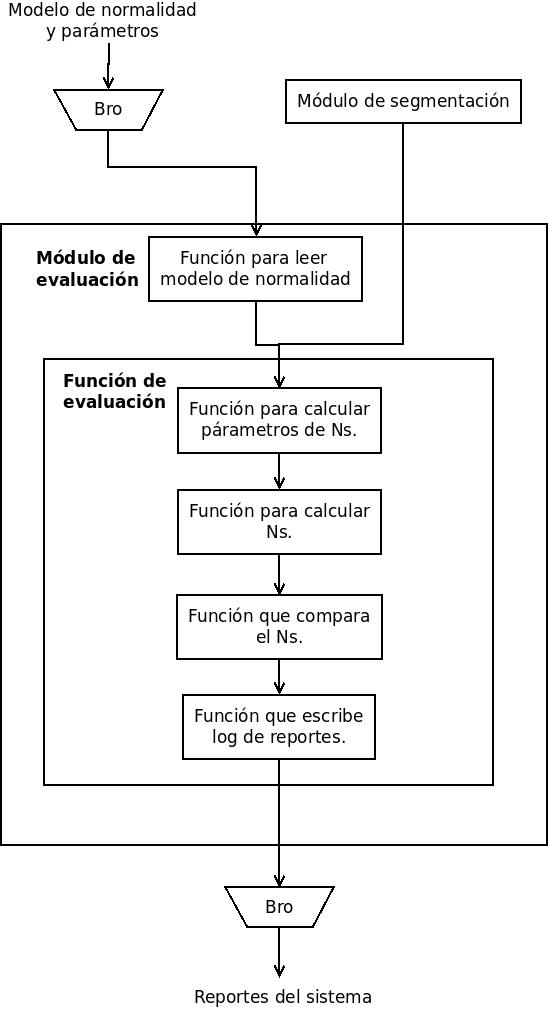
\includegraphics[width=3in]{./img/evalArqui.jpeg}
\caption{Diagrama de bloques del módulo de evaluación.}
\label{fig:arquiEvaluacion}
\end{center}
\end{figure}

\subsubsection{Módulo de Entrenamiento}\label{sec:entrenamiento}

El modelo de normalidad es uno de los aspecto importantes dentro del IDS basado en SSM ya que a partir de la información que este almacena se podrá decidir si un URI es anómalo o no dependiendo de la similitud que posea este con los datos que almacena el modelo. Por esta razón, realizar un modelo de normalidad apropiado es un aspecto  importante para que el módulo de evaluación haga detecciones de intrusiones más certeras.

El módulo encargado de elaborar los modelos de normalidad será el módulo de entrenamiento. A grandes rasgos, este se encargará de recibir un conjunto de segmentos libres de ataques proporcionados por el módulo de segmentación para ir calculando la probabilidad de aparición de cada una de las palabras que aparecen en los mismos, para finalmente, escribir en un archivo toda la información recolectada, es decir, el conjunto de palabras observadas mientras se hacía el entrenamiento, sus probabilidades de aparición y el estado del autómata en el que se observaron las mismas.

Este módulo consta de dos modos: el modo ``Offline'' y el modo ``Online''. La  diferencia fundamental entre el modo ``Online'' y el ``Offline'' es que en el primero necesita como entrada un modelo de normalidad ya construido y los segmentos de URI proporcionados por el módulo de segmentación. Una vez realizado el entrenamiento, esta modalidad se encargará de actualizar el modelo que se leyó al inicio. Por otra parte, el modo ``Online'' solo requiere como entrada los segmentos de URI y como salida proporcionará un  modelo de normalidad construido desde cero.

El modo de entrenamiento ``Offline'' fue dividido en tres funciones. La primera función irá observando los segmentos de los URIs de las peticiones que van llegando y contará el numero de veces que cada segmento fue observado durante el entrenamiento. La segunda función, toma el resultado de las observaciones realizadas por la primera función y calculará la probabilidad de aparición de cada uno de los segmentos haciendo uso de la formula \ref{eq:entrenamiento}. La tercera función tomara los resultados otorgados por la segunda función y los escribirá en un archivo de texto. Este archivo representara el modelo de normalidad construido.

Por otra parte, las tareas a realizar por el modo de entrenamiento ``Online'' fueron divididas de igual modo en tres funciones: La primera función se encargara de leer el modelo de normalidad; la segunda se encargará de tomar el modelo de normalidad leído por la primera función y el conjunto de segmentos de URI del módulo de segmentación. Esta información sera utilizada por la misma para ir calculando la probabilidad de aparición de los segmentos observados. La tercera función se encargara de recibir los resultados obtenidos por la segunda función y actualizara el modelo de normalidad previamente existente.

En la figura \ref{fig:arquiEntrenamiento} se puede apreciar el diagrama de bloques que describe el funcionamiento del módulo de entrenamiento.

\begin{figure}[!htb]
\begin{center}
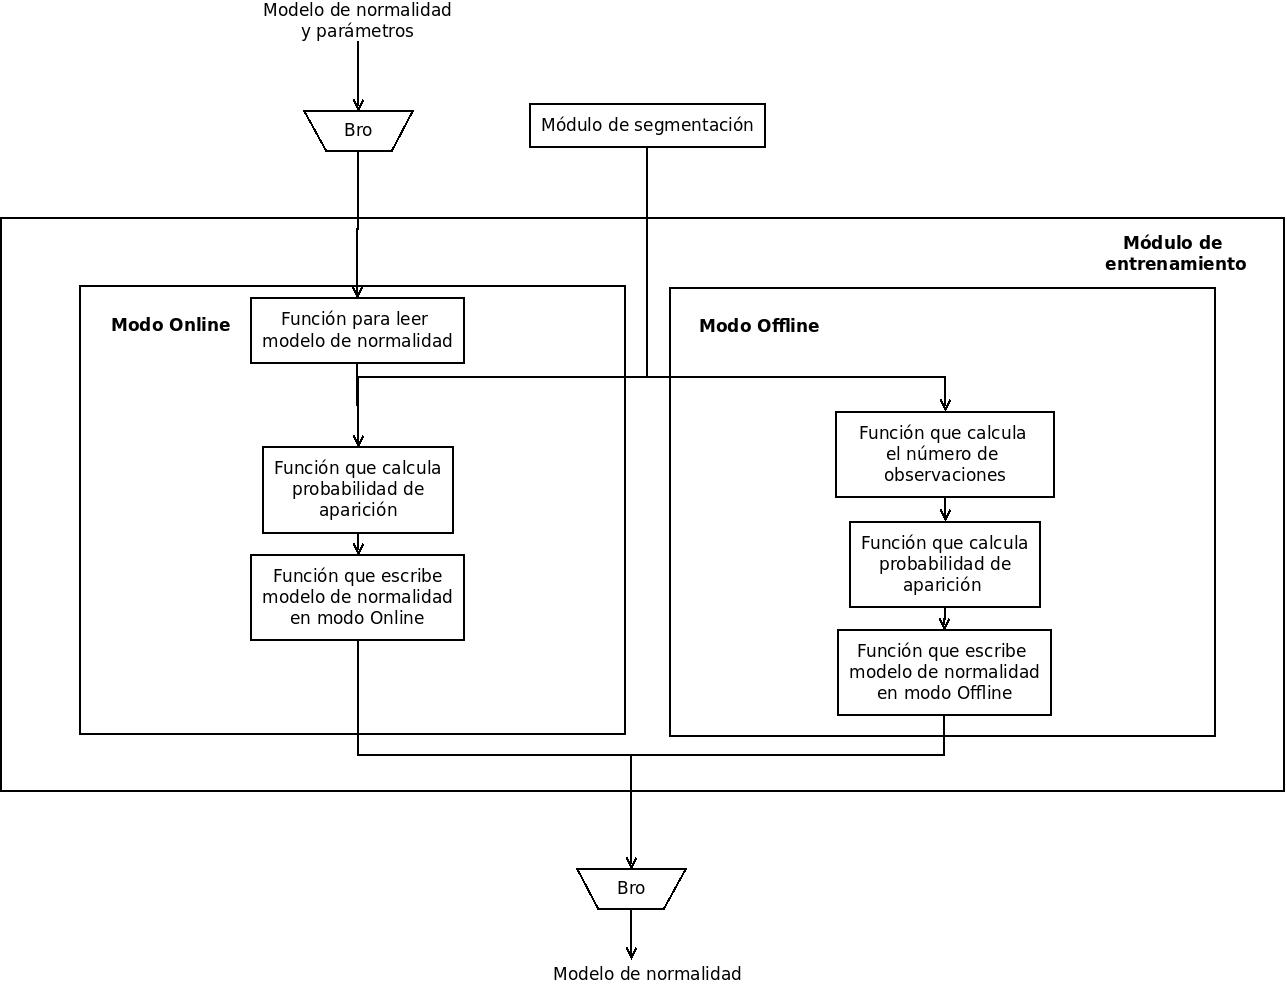
\includegraphics[width=3in]{./img/entrenamArqui.jpeg}
\caption{Diagrama de bloques del módulo de entrenamiento.}
\label{fig:arquiEntrenamiento}
\end{center}
\end{figure}

\section{Implementación del Sistema}

Una vez descrita la arquitectura modular del sistema y las funcionalidades asociadas a los diferentes componentes del sistema, en este capítulo se detallarán las cuestiones más relevantes en cuanto a su implementación.
Así, en primer lugar, se describirán como se implementó el filtro de paquetes HTTP/GET, para luego explicar las estructuras de datos utilizadas por cada uno de los módulos; los parámetros de entrada, salida y la implementación de las funciones que los componen.

\subsection{Filtrado de Paquetes HTTP/GET}

El módulo de segmentación requiere como entrada los URIs extraídos de las peticiones de tipo HTTP/GET. Esta tarea se realizó haciendo uso de las herramientas brindadas por Bro. En concreto, esta funcionalidad fué implementada con un evento primitivo de Bro llamado ``http request''. Este evento se genera y almacena la información de paquetes HTTP cuando son percibidos por dicha herramienta en la red. Su formato es el siguiente:

\textbf{http request}(c: \textbf{connection}, method: \textbf{string}, original\_URI: \textbf{string},
unescaped\_URI: \textbf{string}, version: \textbf{string})
donde:
\begin{itemize}
\item c: es una estructura de datos de tipo ``connection'' que almacena de manera desglosada la información del mensaje HTTP.
\item method: Es el método extraído de la petición (e.g., GET,POST).
\item original\_URI : URI extraído de la petición (sin decodificar).
\item unescaped\_URI : URI extraído de la petición con todas las codificaciones de porcentaje decodificadas.
\item version: Número de la version HTTP (e.g. 1.1). Este estará especificado en la petición.
\end{itemize}

\subsection{Implementación del Módulo de Segmentación}

En esta sección, se explicará de manera detallada la implementación del módulo de segmentación. Este módulo forma parte de los tres que conforman el sistema de detección de intrusiones basado en SSM.

\subsubsection{Función de Segmentación}

En la función de segmentación, el problema que se quiere resolver es el siguiente:construir un analizador sintáctico que haga uso de una gramática (libre de contexto) de atributos que genera el mismo lenguaje que reconoce el autómata presentado en la figura \ref{fig:ssm}. A nivel de implementación lo que se quiere construir es un analizador sintáctico que verifique que los URIs tengan una estructura sintáctica correcta según los estándares del RFC 3986, y que a la vez vaya almacenando los segmentos, delimitados por los delimitadores presentados en la sección \ref{sec:delimitadores}.

A continuación se presentara la forma en que se modeló y se implementó el problema presentado con anterioridad haciendo uso de las herramientas presentadas por el lenguaje de ``scripting'' de Bro.

Para realizar el analizador sintáctico se requiere construir una gramática libre de contexto.

Antes de presentar la gramática se mostrarán los tokens que utilizará la misma como elementos terminales.

Estos tokens utilizarán las expresiones regulares que soporta Bro. Estas están basadas en las expresiones regulares empleadas en Lex, la librería para realizar análisis léxicos del lenguaje de programación C.

La lista de tokens utiliza es la siguiente:

\begin{itemize}
\item protocolo: “http”|”https”
\item host: $(([a-z]+[a-z0-9\-]*[.])?([a-z0-9]+[a-z0-9\-]*[.])+[a-z]{2,3}|localhost)(:([0-9]{1,5}))?|$\\ ((25[0-5]|2[0-4][0-9]|[01]?[0-9][0-9]?)\.){3}(25[0-5]|2[0-4][0-9]|[01]?[0-9][0-9]?)(:([0-9]{1,5}))?
\item elementoPath: [\^?\#]*
\item atributo: [\^\#\&=]
\item valor: [\^\#\&]
\item fragmento: (\#.*)
\end{itemize}

Por otra parte, la gramática libre de contexto en la que está basada la función de análisis sintáctico es la siguiente.

\begin{equation}\label{eq:gramatica}
\begin{aligned}
S -> protocolo “ :// ” H  \\
H -> host “/” P | host \\
P -> P’ “?” Q | P’ “\#” F | P’ \\
Q -> Q’ “\#“ F | Q’ \\
F -> fragment \\
P’ -> \lambda \\
P’ ->  elementoPath \\
P’ -> elementoPath “/” P’ \\
Q’ -> atributo “=” valor \\
Q’ -> atributo “=” valor “\&” Q’ \\
\end{aligned}
\end{equation}

Donde, el elemento de inicio de esta gramática es el símbolo no terminal ``S''

Para almacenar los segmentos en la estructura de datos compuesta de tipo ``UriSegmentado'' que se presenta en la ápendice ~\ref{ssec:estructuraSegmentacion}, a la gramática \ref{eq:gramatica} se le van a asociar atributos a algunas de las reglas de la misma. A este tipo de gramática se le llama gramática de atributos. Los atributos de dicha gramática serán escritos en el lenguaje de ``scripting'' de Bro.

\begin{equation}\label{eq:gramaticaAtributos}
\begin{aligned}
S -> protocolo “ :// ” H { uri\$protocolo := protocolo } \\
H -> host “/” P | host { uri\$host := host  } \\
P -> P’ “?” Q | P’ “\#” F | P’ \\
Q -> Q’ “\#“ F | Q’ \\
F -> fragment { uri\$fragment := fragment } \\
P’ -> \lambda  { uri\$path.append(“”) } \\
P’ ->  elementoPath { uri\$path.append(elementoPath) } \\
P’ -> elementoPath “/” P’ { uri\$path.append(elementoPath) } \\
Q’ -> atributo “=” valor { uri\$query[atributo] := valor } \\
Q’ -> atributo “=” valor “\&” Q’ { uri\$query[atributo] := valor } \\
\end{aligned}
\end{equation}

    La gramática de atributos presentada \ref{eq:gramaticaAtributos} representa el modelo de lo que se implementó haciendo uso de Bro.

    Como Bro no cuenta con una librería propia para programar un parser de manera sencilla, se hizo uso de las herramientas con las que cuenta este para procesar cadena de caracteres y expresiones regulares. Las funciones fundamentales que se utilizaron para implementar  la gramática \ref{eq:gramaticaAtributos} fueron: ``split'', ``split\_all'' y ``decompose\_uri''.

A continuación se explicara un poco el funcionamiento de cada una de ellas.

\begin{itemize}
\item split:
La función ``split'' tiene la siguiente forma:

\textbf{split}(str: \textbf{string}, re: \textbf{pattern}) : \textbf{string\_array Attributes:\&deprecated}

Esta función se encarga de dividir una cadena de caracteres de acuerdo a un patrón e introduce el resultado en un arreglo. Por ejemplo, $split"a-b--cd", /(\-)+/)$ retorna $\{"a", "b", "cd"\}.$

Los parámetros de dicha función son:

\begin{itemize}
\item Str:La cadena de caracteres que se quiere dividir. 
\item Re: El patrón que describe lo delimitadores mediante los cuales será dividida la cadena de caracteres. 
\item Retorna: Un arreglo de caracteres donde cada elemento corresponde a una subcadena de caracteres de Str separado por Re.
\end{itemize}

\item split\_all():
Esta función realiza el mismo trabajo que ``split'' con la diferencia que los separadores son incluidos también el parámetro de salida.  Por ejemplo, $split\_all("a-b--cd", /(\-)+/)$ retorna $\{"a", "-", "b", "--", "cd"\}$.

\item decompose\_uri:
La función decompose\_uri tiene la siguiente forma:

\textbf{decompose\_uri}(uri: \textbf{string}) : \textbf{URI}

decompose\_uri dado un URI, retorna una estructura de datos compuesta de tipo URI que contiene información como el protocolo,la ruta, el número de puerto y los parámetros de las consultas del URI recibido.
\end{itemize}

Por otra parte, para implementar la gramática ~\ref{eq:gramaticaAtributos} se modelaron los elementos no finales de la misma como funciones. Por otra parte, los elementos finales, fueron extraídos haciendo uso de ``split'' y ``split\_all''.

En conclusión, la función encargada de segmentar y realizar el análisis sintáctico del módulo de segmentación posee la siguiente estructura:

\textbf{segmentar}(uri: \textbf{string}) : \textbf{UriSegmentado}.

La función se encargará, de tomar una cadena de caracteres y segmentarla según delimitados por los delimitadores presentados en la sección \ref{sec:delimitadores} y almacenar los mismo en la estructura ``UriSegmentado''.
Los parámetros de dicha función son:
\begin{itemize}
\item url : Cadena de caracteres que será segmentada.
\end{itemize}

\subsubsection{Función de Normalización}

La normalización de los URI debe realizarse de acuerdo a las especificaciones establecidas en la Sección 2.6, habiéndose implementado para ello una función denominada ``normalizar'', con el siguiente formato.

\textbf{normalizar}(url: \textbf{string}): \textbf{string} Donde:

\begin{itemize}
\item url: Variable de tipo ``string'' que será normalizada.
\end{itemize}

Esta función tomará el parámetro de entrada y mediante un ``loop for''
se itera por cada una tabla de hash cuyas claves serían elementos de tipo UTF-8 y los atributos de la misma correspondería a los caracteres sin alguna codificación. Si alguno de los elementos de la tabla está contenido en el ``string'' que la función recibe como entrada, entonces se procederá a reemplazar el elemento del párametro de entrada por el valor que posee dicha clave en la tabla de hash. Esta tarea de sustitución se realizará haciendo uso de la función ``subst string'' que proporciona Bro.

``subst\_string'' es una función de la forma:

\textbf{subst\_string}(s: \textbf{string}, from: \textbf{string}, to: \textbf{string}) : \textbf{string}
Se encarga de hacer sustituciones en una cadena de caracteres. Los
parámetros de esta son:

\begin{itemize}
\item S:Cadena de caracteres en la que se efectúa la sustitución.
\item From: La cadena de caracteres que se va a buscar en ``S'' para ser
sustituida.
\item To: Cadena de caracteres que pasará a sustituir a ``From''.
\end{itemize}


\subsection{Implementación del Módulo de Evaluación}

En esta sección se explicará de manera detallada la manera en la que se implementó el módulo de evaluación explicado en la sección \ref{sec:evaluacion}  haciendo uso del lenguaje de ``scripting'' de Bro.
    
\subsubsection{Modelo de Normalidad en Bro}
\label{sec:lecturaModelo}

En esta sección se explicará cual es el formato de almacenamiento del
modelo de normalidad y los parámetros de configuración, y se explicará como
se implementó la lectura del mismo.

Los elementos que necesitan ser introducidos al módulo de evaluación para su correcto funcionamiento son: el conjunto de observaciones de cada estado (O), el conjunto de vectores de probabilidad de las palabras observadas en cada estado ( $B_{S}, B_{P}, B_{A}, B_{V}$ ), los
valores de probabilidad de fuera de vocabulario ($P_{oovP}, P_{oovA}, P_{oovV}$), y el valor del parámetro $\theta$ (Ec. \ref{eq:ClaseU}).

\subsubsection*{Formato de los Archivos de Entrada}

    Los parámetros necesarios para el funcionamiento del módulo de evaluación, serán introducidos a tráves de dos archivos, un archivo llamado
``config'' que contendrá los valores de la probabilidad de fuera de vocabulario ($P_{oovP}, P_{oovA}, P_{oovV}$ ) y el valor del parámetro $\theta$ (ec. \ref{eq:ClaseU}) y otro llamado
``modeloBro.log'' en el cual estará el conjunto de observaciones de cada estado junto a sus probabilidades de generación.
   
Tanto el archivo ``config'' como el ``modeloBro.log'' están regidos bajo un formato que establece la herramienta de Bro para leer archivos de entrada.

El formato que establece Bro para los archivos de entrada define que la información se debe introducir en columnas separada mediante tabs, y que debe existir un encabezado al inicio del mismo que inicie abriendo con un numeral (\#) seguido de la palabra ``fields''. Luego de esta palabra se escribirán los nombres que se le asignará a cada columna del archivo.

Por lo tanto, el formato del archivo ``config'' sería como el que se muestra en la figura \ref{fig:archivoConfig}.

\begin{figure}[!htb]
\begin{center}
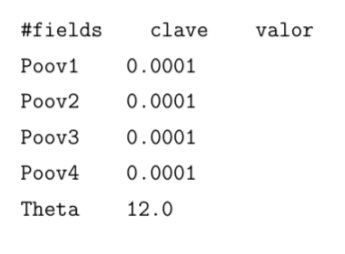
\includegraphics[width=2in]{./img/config.png}
\caption{Formato de archivo ``config''.}
\label{fig:archivoConfig}
\end{center}
\end{figure}	

La primera columna corresponde a las etiquetas que identifican los valores que se encuentran en la segunda columna. Es importante recalcar que los nombres ``Poov1'', ``Poov2'', ``Poov3'', ``Poov4'' y ``Theta'' deben ser escritos en el archivo obligatoriamente de la misma forma en la que aparecen en el ejemplo.

Por otro lado, el formato del archivo ``modeloBro.log'' es el que se muestra en la figura \ref{fig:archivoModeloBro}.

\begin{figure}[!htb]
\begin{center}
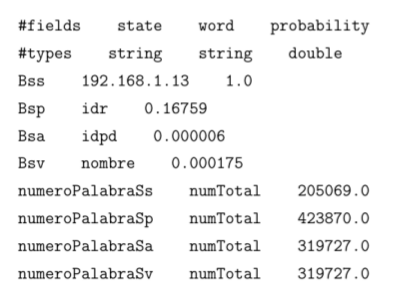
\includegraphics[width=2in]{./img/modeloBro.png}
\caption{Formato de archivo ``modeloBro.log''.}
\label{fig:archivoModeloBro}
\end{center}
\end{figure}	

La segunda columna de este archivo (``word'') corresponde al conjunto de observaciones ``O'' de cada uno de los estados, mientras que la tercera columna (``probability'') indica la probabilidad de aparición de cada palabra ($B_{S}, B_{P}, B_{A}, B_{V}$). Por otra parte, la primera columna (``state'') indica a que estado del autómata \ref{fig:ssm} pertenece cada palabra y su probabilidad de generación.

Las filas del archivo ``modeloBro.log'' que tienen en la primera columna las palabras: ``numeroPalabraSs'', ``numeroPalabraSp'', ``numeroPalabraSa'', ``numeroPalabraSv'' contienen el número de palabras que han sido procesadas por estado. Esta información será utilizada en el entrenamiento en modo ``Offline'' que será explicado en la sección.

\subsubsection*{Lectura de los Archivos}

Una vez explicado el formato de los archivos que contienen los elementos del modelo y los parámetros necesarios para realizar el cálculo y la evaluación del índice de normalidad de los URIs a evaluar se procederá a explicar el funcionamiento de las funciones encargadas de leer los archivos con la información de entrada.

Para leer dicha información se hizo uso del  ``Input Framework'' que otorga Bro como herramienta para leer archivos de entrada. La función utilizada para leer los archivos se llama ``add\_table'' y pertenece al módulo llamado ``Input''.

``add\_table'' se encarga de leer archivos de entrada y almacenar sus datos en una tabla. El formato de esta funcion es el siguiente:\\
%Extraido de : https://www.bro.org/sphinx/frameworks/input.html, https://www.bro.org/sphinx/scripts/base/frameworks/input/main.bro.html\#id-Input::add_table, https://www.bro.org/sphinx/scripts/base/frameworks/input/main.bro.html\#type-Input::TableDescription 
%
\textbf{Input::add\_table}(description: \textbf{Input::TableDescription}) : \textbf{bool} 

Donde ``\textbf{TableDescription}'' es la estructura descrita graficamente en
la figura ~\ref{fig:TableDescription} que se encuentra en el ápendice A.

\subsubsection{Evaluación de las Probabilidades de los URI}

La función ``evaluacion'' del módulo de evaluación, se encargará de hallar el  índice de anormalidad, dado un conjunto de segmentos de URI, e indicará si el mismo es anómalo o no comparándolo con el valor
de $\theta$, para luego escribir los resultados de la evaluación en un archivo de reportes del sistema. La función implementada que se encargara de realizar las tareas anteriormente descritas tiene el siguiente formato:

\textbf{evaluacion}(uriParsed: \textbf{UriSegmentado}, Bvector: \textbf{table[string,string]
of Probability}, config: \textbf{table[string] of Valor})
donde:
\begin{itemize}
\item uriParsed: es un parámetro de tipo ``UriSegmentado'' (figura \ref{fig:uriSegmentado}, ápendice A), que
almacena los segmentos del URI.
\item Bvector: es una tabla que almacena el conjunto de observaciones de cada estado (O) y el conjunto de vectores de probabilidad de las palabras observadas en cada estado, es decir, $B_{S}, B_{P}, B_{A}, B_{V}$.
\item config: Es una tabla que almacena los diferentes Poov y el valor de $\theta$.
\end{itemize}

No obstante, la tarea realizada por ``evaluacion'' fue subdividida en cuatro funciones: ``epsiloSumatoria'', ``calcularIndiceAnormalidad'',
``evaluarIndiceAnormalidad'' y ``escribirReporte''. La función ``epsiloSumatoria'' se encargará de calcular tanto el $\varepsilon_{0}$ que aparece en la expresión \ref{eq:sumB}
como la sumatoria de los logaritmos de los $p_{qtot}$ que se encuentra en la
expresión \ref{eq:Ns}.

El formato de dicha función es el siguiente:

\textbf{epsiloSumatoria}(segmentos: \textbf{UriSegmentado},
Bvector: \textbf{table[string,string] of Probability}, epsilon : \textbf{double}, estado:\textbf{string}):
\textbf{table[count] of double}

donde los parámetros de entrada serán:
\begin{itemize}
\item segmentos: es un parámetro de tipo ``UriSegmentado'' (figura \ref{fig:uriSegmentado}, ápendice A), que
almacena los segmentos del URI.
\item Bvector: es una tabla que almacena el conjunto de observaciones de cada estado (O) y el conjunto de vectores de probabilidad de las palabras observadas en cada estado, es decir, $B_{S}, B_{P}, B_{A}, B_{V}$.
\item epsilon: Valor correspondiente al Poov.
\item estado: estado del autómata que se esta evaluando (``host'',``path'',``argumentos'',
``valores'').
\end{itemize}

El parámetro de salida correspondería a una tabla que contiene dos elementos: el resultado de la suma de las probabilidades de aparición de las
palabras y la suma del los logaritmos de la probabilidad de aparición.

Por otra parte, ``calcularIndiceAnormalidad'', la encargada de calcular
el  índice de anormalidad $N_{s}$ , tiene el siguiente formato:

\textbf{calcularIndiceAnormalidad}(epsilon0: \textbf{double}, N: \textbf{double}, sumaLogaritmos: \textbf{double}) : double. Donde:

\begin{itemize}
\item epsilon0: Valor de $\varepsilon_{0}$ (expresión \ref{eq:sumB}).
\item N: Valor de ``T'' en la expresión (expresión \ref{eq:sumB}).
\item sumaLogaritmos: Suma de los logaritmos de $p_{qtot}$ que se encuentra en la expresión (expresión \ref{eq:sumB}).
\end{itemize}

El parámetro de salida de esta función será el valor del  índice de anormalidad.

La función, ``evaluarIndiceAnormalidad'' que tiene como tarea comparar el  índice de anormalidad ($N_{s}$) con el parámetro $\theta$, de la forma en que se muestra en la expresión \ref{eq:ClaseU} tiene el siguiente formato:

\textbf{evaluarIndiceAnormalidad}(theta: \textbf{double},indiceAnormalidad: \textbf{double})

donde:
\begin{itemize}
\item theta: Umbral de normalidad ($\theta$).
\item indicesAnormalidad: Índice de anormalidad.
\end{itemize}

La ultima función, ``escribirReporte'', la encargada de escribir en el archivo de reportes la información de los URIs que se han detectado como
anómalos presenta el siguiente formato:

\textbf{escribirReporte}(clasificacion: \textbf{string},
uri: \textbf{string},indiceAnormalidad: \textbf{string})

\begin{itemize}
\item clasificacion: En este campo se informa si el URI es anómalo por sobrepasar el umbral de normalidad o por estar construido de manera
incorrecta sintácticamente.
\item uri: En este campo se introduce el URI que se quiere escribir en el
archivo de salida.
\item indiceAnormalidad: Este campo corresponde al índice de anormalidad.
\end{itemize}

La función anterior fue implementada con la ayuda de las herramientas
que aporta el ``Logging Framework'' de Bro y la estructura de datos ``InfoAtaque'' (fig. ~\ref{fig:InfoAtaque}, ápendice A). La funciones del ``Framework'' utilizadas fueron: ``write'' para escribir sobre el archivo y ``create\_stream'' para crearlo. Ambas pertenecen al modulo ``LOG''. 

El formato que sigue la función ``write'' es el siguiente :

\textbf{LOG::InfoAtaque}(id: \textbf{Log::ID}, columns: \textbf{any}) : \textbf{bool}
Sus parámetros de entrada son:

\begin{itemize}
\item id: Es al ID asociado al archivo sobre el cual se va a escribir.
\item column: Registro que contiene los valores que van a ser escritos en el
archivo.
\end{itemize}

El parámetro de salida de esta función es ``verdadero'' si el archivo fue encontrado y no existieron problemas al momento de la escritura, y ``falso'' de
lo contrario.

Por otra parte, la función ``create\_stream'', esta definida de la siguiente
forma:

\textbf{LOG::create stream}(id: \textbf{Log::ID}, stream: \textbf{Log::Stream}) : \textbf{bool}

Los parámetros de entrada de la misma son:

\begin{itemize}
\item id: Es al ID asociado al archivo sobre el cual se va a escribir.
\item stream: Registro que almacenará la ruta en donde se quiere crear el
archivo y la estructura de dato que se utilizará en la escritura del
archivo.
\end{itemize}

El parámetro de salida de esta función sera ``verdadero'' si se puedo crear el
archivo y ``falso'' si es posible.


\subsection{Implementación del Módulo de Entrenamiento}

Como se pudo apreciar en la sección \ref{sec:entrenamiento} el modo de entrenamiento cuenta con dos modos: el modo ``Online'' y el modo ``Offline''. En esta se sección, se explicarán las funciones implementadas en cada uno de ellos.

\subsubsection{Entrenamiento ``Offline''}

El modo de entrenamiento ``Offline'', es el encargado de crear un modelo de normalidad desde cero.Esta modalidad está conformada por una
función general llamada ``entrenarOffline'', que fué subdividida en tres funciones: ``entrenamientoOffline'',
``evaluarProbabilidad'' y ``escribirArchivoOffline''.

``entrenarOffline'', será la función encargada de llamar el resto de las
funciones, necesarias para realizar el entrenamiento en modo ``Offline''. Su
formato es el siguiente:

\textbf{entrenarOffline}(segmentos: \textbf{UriSegmentado})
donde:

\begin{itemize}
\item segmentos: campo de tipo ``UriSegmentado'' (fig. \ref{fig:uriSegmentado}, ápendice A), que almacena los segmentos de un URI
\end{itemize}

Por otra parte, la función ``entrenamientoOffline'' irá observando los segmentos de los URIs de las peticiones que van llegando y contará el número de veces que cada segmento fue observado durante el entrenamiento. El formato de la misma sigue la siguiente estructura:

\textbf{entrenamientoOffline}(segmentos: \textbf{UriSegmentado}, vocabulario: \textbf{table[string] of Entrenamiento}, estado: \textbf{string})
donde:
\begin{itemize}
\item segmentos: campo de tipo ``UriSegmentado'' (fig. ~\ref{fig:uriSegmentado}, ápendice A), que almacena
los segmentos de un URI (las observaciones).
\item vocabulario: Tabla que contiene una lista de palabras y una lista de
números que corresponde al número de apariciones y probabilidad de
aparición de las misma (fig. ~\ref{fig:figEntrenamiento}, ápendice A).
\item numPalabras: Número total de apariciones de todas las palabras vistas durante el entrenamiento de un estado en concreto.
\item estado: estado del autómata que se esta entrenando (``host'', ``path'',
``argumentos'',``valores'').
\end{itemize}

La ``evaluarProbabilidad'' , encargada de tomar el resultado de las observaciones realizadas por ``entrenamientoOffline'' y calcular la probabilidad de aparición de cada uno de los segmentos (ec. \ref{eq:entrenamiento}) tiene el siguiente formato:

\textbf{evaluarProbabilidad}(vocabulario: \textbf{table[string] of Entrenamiento},
numPalabras: \textbf{double})
\begin{itemize}
\item vocabulario: Tabla que contiene una lista de palabras y una lista de
números que corresponde al número de apariciones y probabilidad de
aparición de las misma (fig. ~\ref{fig:figInfo}, ápendice A).
\item numPalabras: Número total de apariciones de todas las palabras vistas durante el entrenamiento de un estado en concreto.
\end{itemize}

Finalmente, ``escribirArchivoOffline'' toma los resultados otorgados por
``evaluarProbabilidad'' y los escribirá en un archivo de texto. El formato de
esta función es el siguiente:

\textbf{escribirArchivoOffline}(vocabulario: \textbf{table[string] of Entrenamiento}, estado: \textbf{string})
donde:
\begin{itemize}
\item vocabulario: Tabla que contiene una lista de palabras y una lista de
números que corresponde al número de apariciones y probabilidad de
aparición de las misma (fig. ~\ref{fig:figInfo}, ápendice A).
\item estado: estado al que pertenece la tabla ``vocabulario''.
\end{itemize}

\subsubsection{Entrenamiento ``Online''}

El modo de entrenamiento ``Online'', encargado de hacer modificaciones a un modelo de normalidad previamente existente fue implementado
haciendo uso de una función llamada ``entrenarOnline'' que a su vez esta
subdividida en tres funciones. Los
nombres que se les dio a estas al momento de ser implementadas fueron:
``entrenamientoOnline'',``escribirArchivoOnline''.

La función ``entrenarOnline'', cuya tarea sera llamar al resto de las funciones del entrenamiento en modo ``Online'' tiene el siguiente formato:

\textbf{entrenarOnline}(uriParsed:\textbf{segmentos::UriSegmentado})
donde:

\begin{itemize}
\item segmentos: campo de tipo ``UriSegmentado'' (fig. \ref{fig:uriSegmentado}, ápendice A), que almacena
los segmentos de un URI
\end{itemize}

Por otra parte, ``entrenamientoOnline'', encargada de calcular la probabilidad de aparición de los segmentos observados haciendo uso de de los segmentos de URI dado por ``entrenarOnline'' y el modelo de normalidad, leído por el módulo de lectura del sistema, sigue el siguiente formato:

\textbf{entrenamientoOnline}(segmentos: \textbf{UriSegmentado},
modelo: \textbf{table[string,string] of Probability}, numPalabras: \textbf{double}, state: \textbf{string})
donde:
\begin{itemize}
\item segmentos: campo de tipo ``UriSegmentado'' (fig. \ref{fig:uriSegmentado}, ápendice A), que almacena los segmentos de un URI.
\item modelo: tabla que almacena el modelo de normalidad previamente
leído.
\item numPalabras:
\item state: nombre del estado al que se le esta realizando el entrenamiento
(``host'',\\``path'',``atributos'',``valores''.
\end{itemize}

Finalmente, ``escribirArchivoOnline'', se encargará de recibir todos los
resultados obtenidos del entrenamiento para escribirlos sobre un archivo de
texto. El formato de esta función es:

\textbf{escribirArchivoOnline}(vocabulario: \textbf{table[string,string] of Probability})
donde:
\begin{itemize}
\item vocabulario: Es una tabla que almacena los resultados del entrena-
miento.
\end{itemize}


\section{Evaluación y Pruebas}

En el presente sección se explicará las pruebas operativas
realizadas al sistema. Así como las bases de datos utilizadas para realizar
las misma.

\subsection{Base de Datos}\label{ssec:DB}

Las bases de datos utilizadas por las pruebas fueron trazas capturadas
en servidores web. Para capturar estos paquetes de tipo HTTP los pasos a
seguir fueron los siguientes:

\begin{enumerate}
\item Se instaló una aplicación de servicio web en el ordenador.
\item Se corrió una aplicación web en la aplicación anteriormente instalada.
\item Se empezaron a hacer solicitudes a la aplicación web a tráves de otro
dispositivo. Mientras esto ocurría, ``Wireshark'' realizaba las capturas
de los paquetes de la red.
\end{enumerate}
Se obtuvo cuatro bases de datos:
\begin{itemize}
\item db1.pcap: Capturas de paquetes provenientes de las solicitudes realizadas a una aplicación web, A.
\item db2.pcap: Capturas de paquetes provenientes de la misma aplicación
web A.
\item db3.pcap: Capturas de paquetes provenientes de una aplicación web,
B.
\item db4.pcap: Capturas de paquetes descargadas de: \cite{wireshark}.
\end{itemize}

\subsection{Pruebas Operativas}

A continuación, se explicaran las pruebas operativas que se les aplicaron
a las tres modalidades del sistema implementado.

\subsubsection{Modo Entrenamiento ``Offline''}

Para probar el modo ``Offline'' del sistema, se tomó la base de datos \textbf{db3.pcap} explicada en la sección \ref{ssec:DB}, y se le ingresó al sistema configurado en modo ``Offline''. Una vez realizado esto, se observó el modelo de
normalidad arrojado por dicha modalidad.
En la figura \ref{fig:modeloOffline} se puede apreciar el modelo de normalidad obtenido
por la misma.

\begin{table}[!htb]
\begin{center}
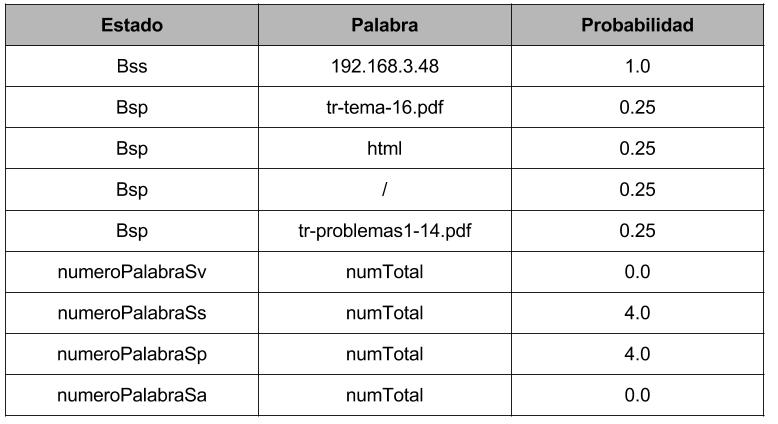
\includegraphics[width=3in]{./img/modeloOffline.jpg}
\caption{Modelo de normalidad obtenido en el modo ``Offline''.}
\label{fig:modeloOffline}
\end{center}
\end{table}

\subsubsection{Modo Entrenamiento ``Online''}

El modo ``Online'' del sistema fue probado ingresando la base de datos \textbf{db4.pcap} explicada en la sección \ref{ssec:DB} al sistema junto con el modelo mostrado en la figura \ref{fig:modeloOffline}. Una vez realizado esto, se observo la salida y se pudo verificar que, en efecto el modelo antiguo fue modificado. En la figura \ref{fig:modeloOnline} se puede apreciar la salida de esta modalidad tras la prueba realizada.

\begin{table}[!htb]
\begin{center}
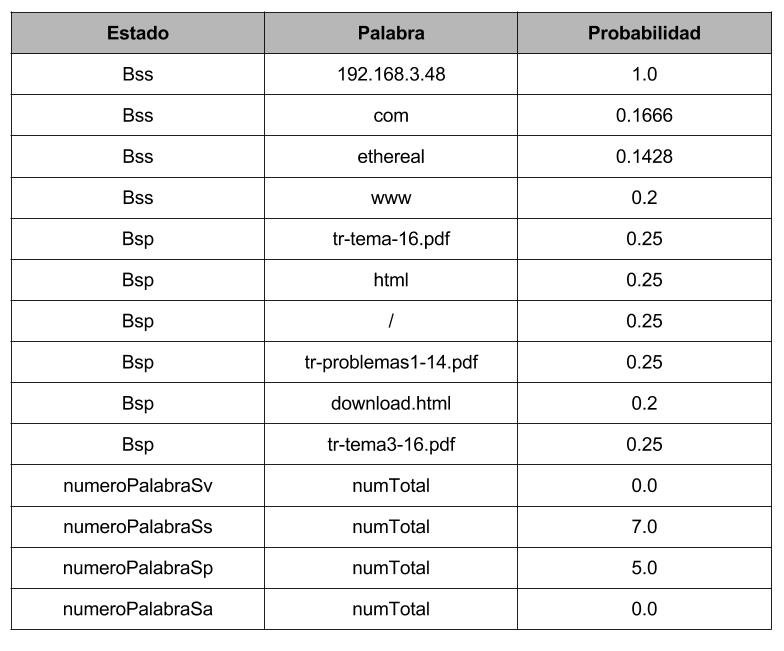
\includegraphics[width=3in]{./img/modeloOnline.jpg}
\caption{Modelo de normalidad obtenido en el modo ``Online''.}
\label{fig:modeloOnline}
\end{center}
\end{table}

\subsubsection{Modo Evaluación}

Para realizar la prueba del modo de evaluación se tomó la base de datos
\textbf{db1.pcap} para realizar un modelo de normalidad haciendo uso del modo de entrenamiento ``Offline''. De esta manera, se evaluarán las trazas que se encuentran en la base de datos, \textbf{db2.pcap} y \textbf{db3.pcap} y se observaran los resultados obtenidos.
La intención de esta prueba es comparar los  índices de anormalidad
obtenidos por la base de datos \textbf{db2.pcap} y \textbf{db3.pcap}.
Como la base de datos \textbf{db2.pcap} posee el mismo comportamiento que
el del modelo de normalidad por pertenecer a peticiones realizadas al mismo servidor, se espera que los  índices de anormalidad sean mas bajos que los obtenido por \textbf{db3.pcap}, ya que esta trazas pertenecen a peticiones que no se encuentran registradas en el comportamiento del modelo de normalidad.
En la figura \ref{fig:indicesMalos} se muestran los resultados de los  índices de anormalidad calculados cuando se evalúa la base de datos \textbf{db3.pcap}.
Se puede observar que los índices oscilan entre 25 y 36.
Por otra parte, en la figura \ref{fig:indicesBuenos} se pueden detallar los índices de anormalidad resultantes, de evaluar la base de datos \textbf{db2.pcap}.Se puede apreciar que los índices de anormalidad de la figura \ref{fig:indicesBuenos} son mas bajos que los de la figura \ref{fig:indicesMalos}. Estos resultados son los esperados, ya que \textbf{db2.pcap} no presenta incongruencias con el modelo de normalidad construido, mientras que la base de dato \textbf{db3.pcap} si. Por lo tanto es conveniente que el sistema lo catalogue como anomalías.
Un parámetro $\theta$, óptimo para esta prueba en particular, debería ser un
valor que sea menor que 25 y mayor que 18.

\begin{table}[!htb]
\begin{center}
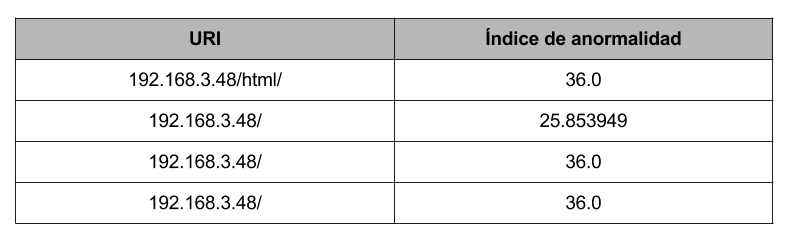
\includegraphics[width=3in]{./img/indicesMalos.png}
\caption{Índices de anormalidad obtenidos de db3.pcap.}
\label{fig:indicesMalos}
\end{center}
\end{table}

\begin{table}[!htb]
\begin{center}
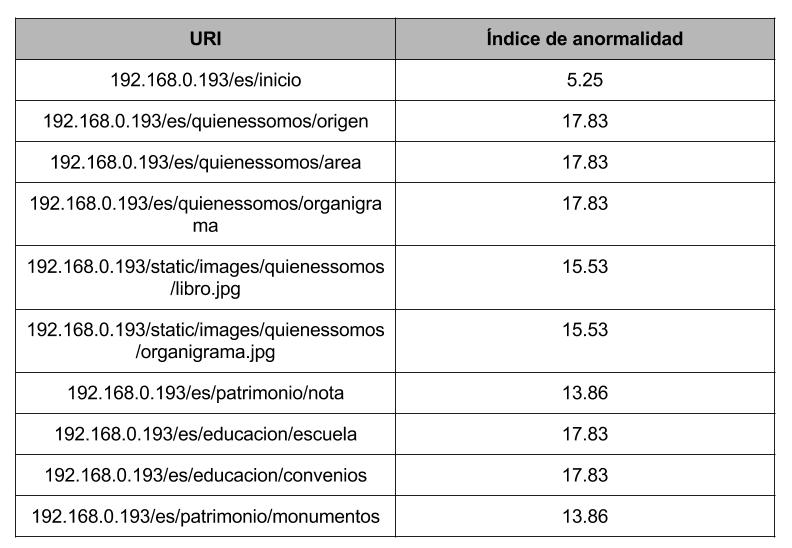
\includegraphics[width=3in]{./img/indicesBuenos.jpg}
\caption{Índices de anormalidad obtenidos de db2.pcap.}
\label{fig:indicesBuenos}
\end{center}
\end{table}
